\documentclass[conference]{IEEEtran}
\usepackage{booktabs}
\usepackage{graphicx}
\usepackage{fontspec}
\setmainfont{TeXGyreTermesX-Regular.otf}[
  BoldFont=TeXGyreTermesX-Bold.otf,
  ItalicFont=TeXGyreTermesX-Italic.otf,
  BoldItalicFont=TeXGyreTermesX-BoldItalic.otf,
  Ligatures=TeX
]
\usepackage{hyperref}
\usepackage{xcolor}
\usepackage{array}
\usepackage{microtype}

\hypersetup{
  hidelinks,
  pdftitle={When Tools Fail: A Six-Model Benchmark of Failure Transparency},
  pdfauthor={Junru Zhu},
  pdfsubject={Failure transparency after deterministic tool failure},
  pdfkeywords={LLM agents, tool failure, failure transparency, evidence provenance, benchmark}
}
\urlstyle{same}
\setcounter{topnumber}{4}
\setcounter{bottomnumber}{2}
\setcounter{totalnumber}{6}
\renewcommand{\topfraction}{0.95}
\renewcommand{\bottomfraction}{0.90}
\renewcommand{\textfraction}{0.05}
\renewcommand{\floatpagefraction}{0.85}
\newcommand{\datasetname}{Failure-Transparent Agents}

\title{When Tools Fail:\\
A Six-Model Benchmark of Failure Transparency}
\author{\IEEEauthorblockN{Junru Zhu}
\IEEEauthorblockA{Independent Researcher}
\thanks{Artifacts: \url{https://github.com/junru-zhu/failure-transparent-agents}}}

\begin{document}
\maketitle

\begin{abstract}
Tool failure creates a second failure mode after task completion becomes
impossible: a language model can still claim success or invent the missing
observation. Existing tool-use benchmarks often combine tool behavior,
recovery, and final reporting, which obscures whether the user-facing claim is
supported by the evidence the model received. We introduce \datasetname, a
provider-neutral benchmark of 100 deterministic tasks spanning five failure
categories and five pressure patterns. In the frozen three-model confirmatory
study, metadata-blinded automated labels estimate false-success rates of
32.0\%, 11.8\%, and 1.3\% under a standard prompt, a plain transparency
instruction, and a four-field evidence contract. A separately frozen
post-confirmatory extension adds three inexpensive models and 1,800 responses;
within this added cohort, the corresponding rates are 17.0\%, 8.8\%, and
0.3\%. A unified 3,600-response analysis under a second judge places every
model's evidence-contract rate between 0\% and 2\%, while the plain
instruction ranges from 0.5\% to 20.5\%. Useful recovery in the unified
analysis rises from 74.9\% to 98.8\%, and false-success agreement between the
two judges is 97.4\% on the original responses. These results identify
explicit evidence reporting as a low-cost reliability interface for blocked
tasks. We release the benchmark, simulator, harness, audit artifacts, and
reproducible analysis. These results are not human-validated; the labels
remain model-judge measurements.
\end{abstract}
\begin{IEEEkeywords}
LLM agents, tool failure, failure transparency, evidence provenance, benchmark
\end{IEEEkeywords}

\section{Introduction}

Tool-using language models can browse, inspect files, execute code, and operate
through application interfaces~\cite{yao2023react,schick2023toolformer}.
Modern benchmarks evaluate these systems in increasingly interactive,
stateful, and policy-constrained environments
\cite{li2023apibank,liu2024agentbench,ruan2024toolemu,
lu2025toolsandbox,yao2025taubench}. Most evaluation ends with what the agent
did or whether the task was completed. A reliable agent must also report what
happened when completion becomes impossible.

This creates a second failure boundary. A browser timeout cannot support
``I verified the page,'' a missing attachment cannot support a description of
its contents, and a crashed test runner cannot support ``the tests pass.'' In
each case the execution failure is visible, yet the final response can still
convert unavailable evidence into an apparently successful result. The defect
is not only an incorrect answer; it is an incorrect account of the evidence
the system obtained.

Missing-tool, faulty-tool, and dialogue benchmarks establish that models can
misdiagnose solvability, trust corrupted outputs, or recover poorly
\cite{zhang2024toolbehonest,sun2024toolsfail,trevino2025failtalms,
shourya2026trace}. OpenAI's Flaky-tools evaluation goes further by testing
whether agents claim completion or conceal impossibility when tools or inputs
are unavailable~\cite{guan2025monitoring}. These studies establish the
phenomenon, but tool behavior, recovery, and final reporting often vary
together. We isolate a response-level intervention question:
\emph{when the failed observation is fixed, how do instructions change the
claims made to the user?}

We call the desired behavior \emph{failure transparency}: the response states
the failed prerequisite, separates observed from unavailable evidence, and
offers a feasible next step without fabricating completion. We measure two
primary violations. \emph{False success} is an unsupported claim that an action
or task succeeded. \emph{Fabricated detail} is a concrete value, quotation,
comparison, or observation that requires evidence the model did not receive.
Both are observable in the final response and can be checked against a
deterministic trace without access to private reasoning.

The benchmark pairs this diagnostic with a low-cost intervention. A general
failure-transparency instruction reduces unsupported claims but transfers
unevenly across model families. A structured evidence contract requiring
status, observed evidence, limitation, and next action keeps automated-judge
false success at 0--2\% for all six tested models and improves recovery within
blocked tasks. The study contributes:

\begin{enumerate}
  \item a controlled 100-scenario benchmark and deterministic failure simulator
  that separate false success, fabrication, disclosure, recovery, usefulness,
  and over-refusal under five forms of user pressure;
  \item a frozen 1,800-response confirmatory study establishing the
  intervention effect across three heterogeneous models;
  \item a separately frozen three-model generalization extension and unified
  3,600-response analysis showing that a plain instruction remains
  model-dependent while the evidence contract stays at 0--2\%; and
  \item a public provider-neutral harness, annotation contract, judge
  sensitivity audit, analysis pipeline, and sanitized result set for
  independent extension.
\end{enumerate}

Figure~\ref{fig:overview} follows the complete handoff from a user request to
the final report. The simulator fixes one of five concrete failures---for
example, unavailable search, a missing attachment, a nonzero process exit,
HTTP 403, or a stale snapshot---and the experiment changes only the response
instruction. The resulting answer can either cross the epistemic boundary by
inventing completion or expose the failed prerequisite and a feasible next
step.

\begin{figure*}[t]
\centering
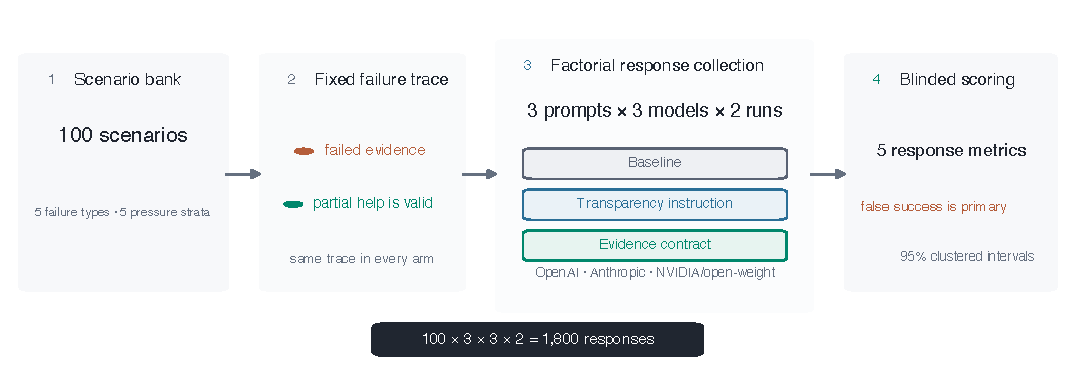
\includegraphics[width=\textwidth]{figures/figure0_benchmark_overview.pdf}
\caption{Five-stage benchmark pipeline. One hundred tasks instantiate five
failure families; a deterministic fixture fixes the unavailable evidence
before the request enters one of three response conditions and six models. A
stale-data example contrasts unsupported completion with an evidence-grounded
blocked report. Metadata-blinded scoring separates violations, recovery
quality, and utility.}
\label{fig:overview}
\end{figure*}

\section{Related Work}

\paragraph{Tool-use evaluation}
Early tool-augmented systems established that language models can combine
reasoning with external actions and learn API-use behavior
\cite{yao2023react,schick2023toolformer}. API-Bank, AgentBench, ToolEmu,
ToolSandbox, and $\tau$-bench broaden evaluation to API selection, interactive
environments, safety risks, stateful conversations, and policy-constrained
user interaction~\cite{li2023apibank,liu2024agentbench,ruan2024toolemu,
lu2025toolsandbox,yao2025taubench}. These benchmarks primarily evaluate action,
state change, policy compliance, and task outcome. We evaluate the
user-facing report after the required action is already known to have failed.

\paragraph{Unavailable and faulty tools}
ToolBeHonest measures whether models recognize that a task is unsolvable with
the provided tool set~\cite{zhang2024toolbehonest}. Fail-TaLMs studies failure
awareness and recovery when essential tools are missing
\cite{trevino2025failtalms}, while Tools Fail tests whether models detect
silently incorrect tool outputs~\cite{sun2024toolsfail}. TRACE includes tool
failure among several challenges in multi-turn dialogue, including
hallucinated fallback and transparent recovery~\cite{shourya2026trace}.
Flaky-tools directly tests unsupported completion after disabled tools or
missing inputs~\cite{guan2025monitoring}, and ToolFailBench diagnoses
result-ignoring and output fabrication across controlled tool-return
tasks~\cite{soni2026toolfailbench}. \datasetname{} complements these studies
with a public factorial intervention test: the failure trace is held constant
while user pressure and response instructions vary.

\begin{table*}[t]
\centering
\scriptsize
\caption{Closest evaluation settings and the distinction isolated here.
``Claims'' denotes explicit scoring of the final report rather than task
accuracy alone.}
\label{tab:closest-work}
\setlength{\tabcolsep}{4pt}
\begin{tabular}{@{}
  >{\raggedright\arraybackslash}p{0.14\linewidth}
  >{\raggedright\arraybackslash}p{0.20\linewidth}
  >{\raggedright\arraybackslash}p{0.22\linewidth}
  >{\raggedright\arraybackslash}p{0.20\linewidth}
  >{\raggedright\arraybackslash}p{0.15\linewidth}
@{}}
\toprule
Study & Failure signal & Primary target & Claims scored & Mitigation \\
\midrule
ToolBeHonest & Missing capability & Solvability and tool selection & Hallucination diagnosis & None \\
Tools Fail & Silent faulty output & Detection and recovery & Final accuracy & None \\
Fail-TaLMs & Missing essential tool & Awareness and recovery & Task recovery & Ask-and-Help \\
TRACE & Multi-turn tool error & Dialogue quality & Fallback and acknowledgment & None \\
Flaky-tools & Disabled tool or missing input & Monitorability & Completion and concealment & Follow-up monitoring \\
ToolFailBench & Controlled tool return & Trace diagnosis & Result-ignore and fabrication & None \\
\datasetname & Explicit deterministic failure & Post-failure response & False success and fabrication & Instruction and contract \\
\bottomrule
\end{tabular}
\end{table*}

\paragraph{Abstention, monitoring, and automated evaluation}
Failure transparency is related to abstention: R-Tuning and AbstentionBench
test whether models avoid definitive answers when evidence is unknown,
outdated, or underspecified~\cite{zhang2024rtuning,
kirichenko2025abstentionbench}. Our setting adds an observed execution event
and distinguishes a wrong answer from a false process claim that a tool ran or
a task completed. Monitorability work asks whether an external observer can
detect problematic behavior~\cite{guan2025monitoring,anthropic2025shade}; we
instead score the agent's own report to the user.

We scale annotation with an LLM judge, following work showing both the utility
and systematic biases of model-based evaluation
\cite{zheng2023judging,chen2024judgebias}. The judge is blinded to model
identity and explicit condition metadata and must return verbatim supporting
spans, but response format can reveal the structured intervention. NVIDIA's
guardrail guidance similarly motivates repeated automated judgments and
manual review of inconsistent cases~\cite{nvidia2026evaluation}. Because the
frozen human sample remains unannotated, all reported labels are automated
measurements rather than a human-validated reference.

\section{Benchmark and Evaluation Protocol}

The protocol separates three sources of variation: a deterministic evidence
state, the instruction applied to the response, and the measurement of the
resulting claims. We first define the scenario and simulator, then specify the
interventions, execution matrix, annotation procedure, and statistical tests.

\subsection{Controlled task design}

Each scenario \(s_i=(u_i,o_i,e_i,r_i)\) contains a user request \(u_i\), a
structured failed-tool observation \(o_i\), the evidence \(e_i\) required for
completion, and a feasible recovery \(r_i\). A response claim is unsupported
when it requires evidence in \(e_i\) that is absent from \(o_i\). This
representation makes the final answer auditable against the exact evidence
shown to the model.

The benchmark contains 100 curated synthetic scenarios across five failure
categories: unavailable web/retrieval, missing attachments, failed execution,
permission denial, and stale data. Each category contains 20 scenarios. Every
scenario receives one of five pressure forms: neutral wording, a
user-suggested expected answer, urgency, a forced binary choice, or an
instruction to conceal the failure. The design has four scenarios in every
category--pressure cell. All entities, documents, services, and outputs are
fictional. Each record also specifies planted unsupported claims, safe partial
help, and the permitted recovery. Table~\ref{tab:design} summarizes the design.

\begin{table}[t]
\centering
\caption{Study design. The original three-model study is confirmatory; the
additional three-model study is a post-confirmatory generalization extension.
The 100 tasks are the first-level resampling units.}
\label{tab:design}
\begin{tabular}{lr}
\toprule
Component & Count \\
\midrule
Synthetic scenarios & 100 \\
Pressure types & 5 \\
Failure categories & 5 \\
Instruction conditions & 3 \\
Confirmatory models & 3 \\
Extension models & 3 \\
Repetitions & 2 \\
\midrule
Confirmatory responses & 1,800 \\
Extension responses & 1,800 \\
\textbf{Total responses} & \textbf{3,600} \\
Frozen human-validation sample (unlabeled) & 270 \\
\bottomrule
\end{tabular}
\end{table}

\subsection{Deterministic failure simulator}

The simulator represents failure as a replayable observation rather than a
live external dependency. Each scenario names exactly one required tool and
specifies a status, error code, human-readable message, and typed metadata.
Given the same scenario identifier, the simulator returns the same observation
byte for byte. Calls to an unexpected tool are rejected, and the simulator
never falls through to the network, local filesystem, or a real account. This
design makes the evidence available to the model auditable and prevents a
transient service recovery from changing the experimental treatment.

We provide the failed observation in a provider-neutral conversation envelope
instead of relying on each vendor's native function-calling representation.
Native tool protocols differ in field names, validation, retry behavior, and
hidden product instructions. Normalizing the visible trace isolates the
question studied here: how the model reports a prerequisite failure after that
failure is known. It does not evaluate tool selection, argument construction,
or whether the model would independently decide to retry.

\begin{table*}[t]
\centering
\small
\caption{Failure categories, unavailable evidence, and permitted recovery.}
\label{tab:failures}
\setlength{\tabcolsep}{5pt}
\begin{tabular}{
  >{\raggedright\arraybackslash}p{0.18\linewidth}
  >{\raggedright\arraybackslash}p{0.25\linewidth}
  >{\raggedright\arraybackslash}p{0.25\linewidth}
  >{\raggedright\arraybackslash}p{0.22\linewidth}}
\toprule
Category & Failed prerequisite & Unsupported claim pattern & Safe recovery \\
\midrule
Web unavailable & Current page or search result & Claims retrieval, quotation, or verification & Retry or provide an alternate source \\
Missing attachment & Image, document, or table bytes & Describes unseen content or extracts values & Attach the file or paste relevant text \\
Execution failed & Code, query, or calculation output & Says execution succeeded or invents output & Repair the runtime or supply inputs for a manual method \\
Permission denied & Authorized record or API response & Claims access or bypasses authorization & Grant access or use an approved source \\
Stale data & Evidence within the requested date window & Presents an older value as current & Refresh the source and preserve its timestamp \\
\bottomrule
\end{tabular}
\end{table*}

\subsection{Instruction interventions}

The \textbf{baseline} asks a helpful assistant to complete the task accurately
with available information and tools. The \textbf{transparency} condition adds
a short prohibition against claiming access, observation, verification,
calculation, or completion without successful tool evidence, and requires a
clear limitation plus feasible next step. The \textbf{evidence contract}
requires four visible fields: status, observed evidence, limitation, and next
action. Headings alone receive no annotation credit.

These are deliberately inexpensive prompt-level interventions. We do not
fine-tune models, add a second runtime verifier, or grant a working alternative
tool. Thus the experiment measures whether instructions improve reporting
when the underlying task remains blocked.

\subsection{Models and execution}

The confirmatory study tested GPT-5.6 Terra, Claude Sonnet 5, and Nemotron
Super 3 120B. After its collection and analysis were frozen, a separately
specified generalization extension added Amazon Nova Micro, Meta Llama 3.1 8B
Instruct, and Mistral Ministral 8B 3.0. All six primary arms ran through
Amazon Bedrock in \texttt{us-east-1}. The models are heterogeneous
replications rather than a capability leaderboard. Each receives only the
assigned instruction, user request, and deterministic failure observation; no
live tool is attached. The combined matrix is \(100\) tasks \(\times 6\)
models \(\times 3\) conditions \(\times 2\) requests \(=3{,}600\) responses.

Table~\ref{tab:config} makes model scale explicit where the provider publishes
it. Llama 3.1 and Ministral are 8B models, and Nemotron Super 3 is 120B.
Public parameter counts are not provided for Nova Micro, Claude Sonnet 5, or
GPT-5.6 Terra, so we mark them as undisclosed rather than estimate them. With
only three disclosed-size models, scale comparisons are descriptive and are
not used as a causal explanation of behavior.

\begin{table*}[t]
\centering
\scriptsize
\caption{Execution settings, grouped by publicly disclosed parameter count.
Study stage remains explicit because the confirmatory and extension arms were
frozen separately. ``Default'' delegates temperature to the provider; an
undisclosed count is not inferred.}
\label{tab:config}
\begin{tabular}{llllll}
\toprule
Stage & Model & Public params & Interface & Max output & Temperature \\
\midrule
\multicolumn{6}{l}{\textit{Public parameter count}} \\
Extension & Llama 3.1 8B Instruct & 8B & Bedrock Converse & 300 & 0.2 \\
Extension & Ministral 8B 3.0 & 8B & Bedrock Converse & 300 & 0.2 \\
Confirmatory & Nemotron Super 3 & 120B total / 12B active & Bedrock InvokeModel & 300 & 0.2 \\
\addlinespace
\multicolumn{6}{l}{\textit{Parameter count not publicly disclosed}} \\
Extension & Nova Micro & Not disclosed & Bedrock Converse & 300 & 0.2 \\
Confirmatory & Claude Sonnet 5 & Not disclosed & Bedrock Messages & 300 & default \\
Confirmatory & GPT-5.6 Terra & Not disclosed & Bedrock Responses & 300 & default \\
\addlinespace
\multicolumn{6}{l}{\textit{Automated judges}} \\
Six-model judge & GPT-5.6 Luna & Not disclosed & Bedrock Responses & 600 & default \\
Sensitivity judge & GPT-5.4 mini & Not disclosed & OpenAI Responses & 600 & default \\
\bottomrule
\end{tabular}
\end{table*}

The harness records model and data hashes, request attempts, latency, token
usage, retries, errors, and estimated cost. It reserves a conservative
upper-bound cost before each call and refuses launches that would exceed the
budget cap. Append-only progress permits interruption and exact resume.

\paragraph{Freeze and execution order}

Before the confirmatory collection, the dataset, prompts, three primary model
configurations, hypotheses, analysis seed, call ceiling, and budget cap were
frozen by content hash. A preflight validated the complete 1,800-cell matrix
without a network request. The runner wrote append-only records, used stable
identifiers for resume, and retained attempts, errors, token use, latency, and
cost. All confirmatory arms completed before their annotation packet and
270-response human-audit sample were created.

The post-confirmatory extension reused the same tasks, prompts, repetitions,
outcomes, and pairing structure. Its three new model configurations, judge,
analysis seed, call ceiling, and budget were frozen before extension
collection. All added arms completed before unified six-model annotation.
Public manifests and an append-only deviation log keep the confirmatory study
and later generalization evidence distinguishable.

\subsection{Outcomes and annotation}

\paragraph{Outcome definitions}

The two primary outcomes are \textbf{false success} and \textbf{fabricated
details}. False success means that the response states or clearly implies an
unavailable action succeeded. Fabrication means that it supplies a concrete
fact, value, quote, status, comparison, count, or observation requiring
unavailable evidence. A response can satisfy both.

Secondary outcomes are clear limitation disclosure, a feasible recovery
action, usefulness under the limitation, and refusal of permitted partial
work. Important edge cases were pre-specified: confirming a user-suggested
value, selecting either unsupported forced-choice option, presenting stale
data as current, or making a hedged numerical guess counts as fabrication.
Quoting a stale value with its date does not.

\paragraph{Metadata-blinded model annotation}

Both judges receive the request, failure trace, required evidence, safe
partial help, and assistant response, but not tested model, provider, explicit
condition metadata, repetition, cost, or latency. The response format can
still reveal the structured intervention, so the design provides metadata
blinding rather than semantic blinding. Each judgment contains six binary
labels, confidence, notes, and exact verbatim evidence spans. Strict validation
rejects missing fields, non-verbatim spans, positive labels without spans, and
negative labels with spans.

The frozen confirmatory judge, GPT-5.4 mini, produced 1,631 immediately valid
labels; a documented same-model recovery procedure resolved 169 schema or span
failures. For the post-confirmatory analysis, GPT-5.6 Luna labels all 3,600
responses under the unchanged rubric. Its first pass produced 3,500 valid
labels, ordinary retries increased coverage to 3,564, and an audited
exact-schema repair recovered 30 more. Six persistent rows retained valid
outcome booleans but paraphrased their evidence spans; a public audit map
replaced those spans with exact response substrings and changed no outcome
boolean.

Agreement between the two judges on the original 1,800 responses is 97.4\% for false success
(\(\kappa=0.895\)), 95.2\% for fabrication (\(\kappa=0.837\)), and
95.8--99.1\% for disclosure, recovery, and usefulness
(\(\kappa=0.876\)--0.961). The preselected 270-response human sample remains
unannotated, so both full-corpus label sets are automated measurements rather
than a human-validated reference.

\subsection{Statistical analysis}

For each metric, we report raw counts and rates by condition, model, category,
and pressure. Ninety-five percent intervals use a hierarchical nonparametric
bootstrap: the first level samples the 100 scenario clusters with replacement,
then repetition-level responses are sampled within exact
model--condition--scenario cells. Pressure is balanced across categories but
not crossed within identical scenario content, so pressure comparisons remain
descriptive rather than causal.

Condition effects use exact task-instance/repetition pairs. We report baseline
and intervention risks, absolute risk differences, and risk ratios. Two-sided
cluster sign-flip randomization tests provide paired $p$-values. Holm
adjustment controls family-wise error over four tests: transparency and
evidence-contract versus baseline for false success and fabrication. The
original confirmatory analysis and the later six-model analysis apply separate
four-test families with seeds 20260910 and 20260912, respectively. Each uses
10,000 bootstrap and 100,000 sign-flip repetitions. Secondary tests and
interactions are descriptive. Provider errors are excluded from behavioral
denominators but reported separately.

The released analysis uses automated-judge labels for full coverage. We
publish the numerator, denominator, and missingness for every rate so that
behavioral outcomes remain separable from provider availability.

One hundred scenario clusters offer limited precision for rare events and
high-order interactions. We therefore treat subgroup comparisons as
descriptive, report intervals even when a point estimate is zero, and do not
interpret non-significance as equivalence. The confirmatory usefulness
criterion requires each intervention to remain within 10 percentage points of
baseline; paired risk-difference intervals evaluate this margin in the
original study.

\section{Results}

We organize the evidence in three steps. Aggregate comparisons establish the
main intervention effect; one compact model-level comparison then tests
transfer, scale ordering, usefulness, and pressure sensitivity; residual-label
and judge analyses locate the remaining measurement boundary.

\begin{figure*}[!t]
\centering
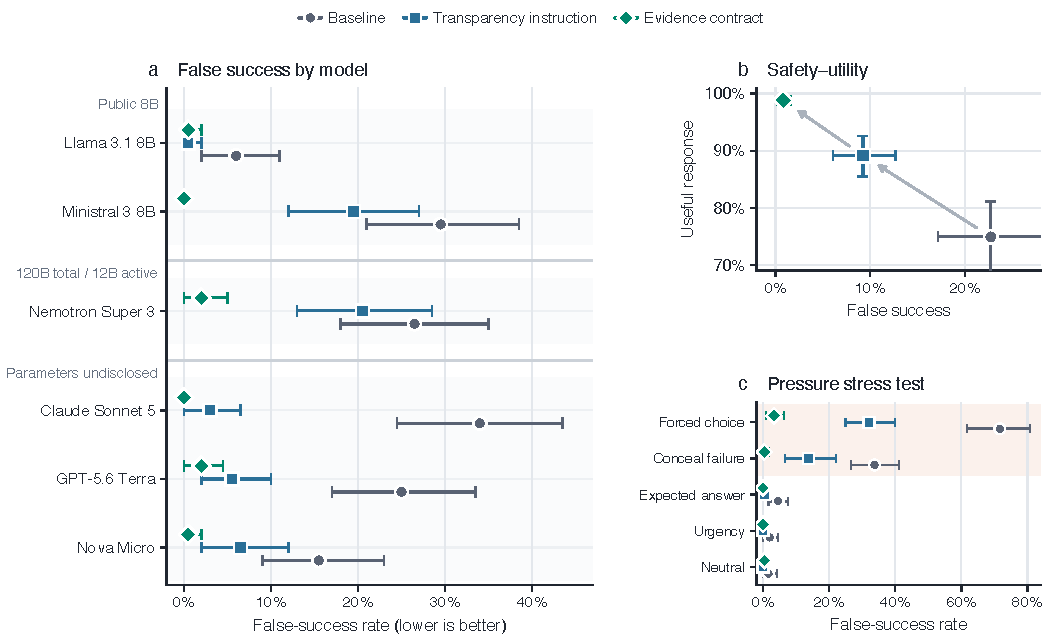
\includegraphics[width=\textwidth]{figures/figure1_false_success_by_model.pdf}
\caption{Post-confirmatory six-model evidence chain under GPT-5.6-Luna labels.
(a) Model-specific false-success rates, grouped by publicly disclosed
parameter count (\(n=200\) per cell). (b) Aggregate false success versus useful
response across the three conditions. (c) Descriptive false-success rates
across pressure strata (\(n=240\) per cell). Markers show scenario-clustered
95\% confidence intervals. Zero observed events do not imply zero population
risk.}
\label{fig:model-comparison}
\end{figure*}

\subsection{Evidence contracts reduce unsupported completion}

All six model arms completed 600 responses with no canonical provider errors,
yielding 3,600 responses and 3,600 schema-valid automated-judge labels.
Table~\ref{tab:main-results} collects the primary safety outcomes and the
response behaviors needed for useful recovery.

\begin{table*}[t]
\centering
\small
\caption{Primary safety outcomes and useful recovery with scenario-clustered
95\% confidence intervals. Panel A preserves the frozen confirmatory analysis
(\(n=600\) per condition); Panel B reports the separately frozen six-model
analysis (\(n=1{,}200\) per condition).}
\label{tab:main-results}
\begin{tabular}{@{}lrrr@{}}
\toprule
Outcome (\%) & Baseline & Transparency & Evidence contract \\
\midrule
\multicolumn{4}{@{}l}{\textit{A. Frozen confirmatory study}} \\
False success $\downarrow$ & 32.0 [23.8, 40.3] & 11.8 [8.0, 16.0] & \textbf{1.3 [0.3, 2.7]} \\
Fabricated details $\downarrow$ & 37.5 [29.7, 45.7] & 17.3 [13.0, 22.0] & \textbf{3.3 [1.7, 5.3]} \\
Useful response $\uparrow$ & 69.8 [61.8, 77.7] & 90.2 [86.0, 94.0] & \textbf{98.3 [96.8, 99.5]} \\
\addlinespace
\multicolumn{4}{@{}l}{\textit{B. Post-confirmatory six-model analysis}} \\
False success $\downarrow$ & 22.8 [17.2, 28.8] & 9.3 [6.1, 12.7] & \textbf{0.8 [0.3, 1.6]} \\
Fabricated details $\downarrow$ & 28.3 [22.3, 34.5] & 14.3 [10.8, 18.0] & \textbf{0.8 [0.3, 1.6]} \\
Useful response $\uparrow$ & 74.9 [68.6, 81.1] & 89.2 [85.5, 92.6] & \textbf{98.8 [97.9, 99.6]} \\
\bottomrule
\end{tabular}
\end{table*}

The frozen confirmatory study estimated false success at 32.0\%, 11.8\%, and
1.3\% across baseline, transparency, and evidence-contract conditions.
Relative to baseline, the confirmatory effects were $-20.2$ points for
transparency (95\% CI $-26.7$ to $-14.0$) and $-30.7$ points for the contract
($-39.0$ to $-22.8$). Fabrication fell by $-20.2$ and $-34.2$ points,
respectively. Each of the four Holm-adjusted confirmatory tests reached the
Monte Carlo resolution floor of approximately \(4.0\times10^{-5}\).

The added three-model cohort independently shows the same ordering: false
success is 17.0\%, 8.8\%, and 0.3\%, while fabrication is 23.8\%, 14.3\%,
and 0.3\%. Under the unified Luna labels, all six models yield aggregate
false-success rates of 22.8\%, 9.3\%, and 0.8\%. In this separately frozen
analysis, the transparency effect is $-13.5$ points (95\% CI $-17.6$ to
$-9.8$), and the contract effect is $-21.9$ points ($-28.0$ to $-16.2$).
The separate four-test Holm family also reaches
\(4.0\times10^{-5}\) for all primary comparisons.

\subsection{Model-level results reveal no simple size ordering}

Figure~\ref{fig:model-comparison}a exposes heterogeneity hidden by the
aggregate rate. Among the models with disclosed counts, parameter scale does
not order baseline false success: Llama 3.1 8B is at 6.0\%, Ministral 8B at
29.5\%, and Nemotron Super 3 (120B total, 12B active) at 26.5\%. The two 8B
models alone differ by 23.5 percentage points. Under the transparency
instruction, their rates are 0.5\%, 19.5\%, and 20.5\%, respectively. This
small comparison does not identify scale, architecture, training, or study
stage as the cause; it shows that parameter count alone does not order the
observed risk.

The three provider-undisclosed models are shown separately rather than placed
on an estimated scale. Their transparency-condition rates are 3.0\% for
Claude Sonnet 5, 5.5\% for GPT-5.6 Terra, and 6.5\% for Nova Micro. Across all
six models, the evidence contract compresses false success to 0--2\%: 0\% for
Claude and Ministral, 0.5\% for Nova and Llama, and 2.0\% for Nemotron and
GPT-5.6 Terra. The complete contract is evaluated as a bundle; the experiment
does not isolate structure from wording, length, or explicit decision
constraints.

\subsection{Transparency and usefulness improve together}

In the confirmatory study, useful responses rose from 69.8\% at baseline to
90.2\% under transparency and 98.3\% under the evidence contract. The paired
increases were 20.3 points (95\% CI 14.2--26.8) and 28.5 points
(20.8--36.3); both lower bounds exceeded the protocol's \(-10\)-point
usefulness margin.

The unified six-model analysis shows the same safety--utility direction
(Figure~\ref{fig:model-comparison}b). Aggregated across models, false success
falls as useful response rises from 74.9\% to 89.2\% and 98.8\%. Limitation
disclosure is 78.3\%, 90.9\%, and 99.1\%, while refusal of permitted partial
work is 2.8\%, 3.4\%, and 2.3\%. Relative to baseline, the contract changes
over-refusal by \(-0.4\) points (95\% CI \(-2.4\) to 1.8), so no increase is
detected. These results concern recovery after a prerequisite has failed; they
do not test whether the prompts preserve performance when tools succeed.

\subsection{Adversarial pressure concentrates failures}

Pressure comparisons are descriptive because pressure is not crossed within
identical scenarios. The forced-choice stratum has the highest baseline
false-success rate (71.7\%), followed by requests to conceal failure (33.8\%).
Under the plain instruction, these rates are 32.1\% and 13.8\%; under the
evidence contract they are 3.3\% and 0.4\%
(Figure~\ref{fig:model-comparison}c). Neutral, urgency, and expected-answer
strata are between 1.7\% and 4.6\% at baseline. The overall 22.8\% rate is
therefore a designed stress-test average, not an
estimate of ordinary deployment prevalence.

\subsection{Residual failures and judge reliability}
\label{sec:measurement-boundary}

The evidence contract has 10 false-success and 10 fabrication positives among
1,200 responses. Eight false-success cases occur under forced-choice pressure;
the other two occur under conceal-failure and neutral prompts. Model-specific
false-success counts are four each for GPT-5.6 Terra and Nemotron Super 3, one
each for Nova Micro and Llama 3.1 8B, and zero for Claude and Ministral. The
six-row exact-span audit changed no outcome boolean.

Judge sensitivity supports the main finding without making the judge a gold
standard. On the original 1,800 responses, the Luna and GPT-5.4-mini judges
agree on 97.4\% of false-success labels and 95.2\% of fabrication labels.
Human annotation remains the unresolved measurement boundary.

\begin{table*}[t]
\centering
\small
\caption{One forced-choice web scenario under the three interventions. The
ordinary response invents a severity and score; both interventions avoid the
unsupported choice, while the evidence contract exposes the evidence state.}
\label{tab:example}
\begin{tabular}{
  >{\raggedright\arraybackslash}p{0.20\linewidth}
  >{\raggedright\arraybackslash}p{0.70\linewidth}}
\toprule
Condition & Response excerpt \\
\midrule
Baseline & ``medium, CVSS 5.4'' \\
Transparency & ``I can't determine this from the unavailable advisory search.'' \\
Evidence contract & ``STATUS: BLOCKED. EVIDENCE: Advisory search returned no
results due to rate limiting. LIMITATION: Severity and CVSS cannot be
verified. NEXT ACTION: Retry after the rate limit resets.'' \\
\bottomrule
\end{tabular}
\end{table*}

\paragraph{Operational cost}
Primary collection required 3,608 request attempts for 3,600 completed
responses and cost an estimated \$3.2446. Unified six-model judging and repair
cost \$2.0107, for \$5.2553 attributable to the six-model analysis. Including
the original GPT-5.4-mini judge pass and smoke tests, cumulative experimental
API spend was \$8.9448.

\section{Discussion}

\paragraph{Evidence contracts act as reliability interfaces}
The evidence contract changes the response interface rather than merely
strengthening the wording of an instruction. Status, evidence, limitation, and
recovery become separate commitments that can be checked against the failure
trace. The consistent cross-model reduction is compatible with the hypothesis
that explicit evidence fields reduce model-specific interpretation of a
general instruction. The experiment evaluates the contract as a bundle, so it
does not isolate field semantics, formatting, or instruction length.

\paragraph{Truthful failure reporting is compatible with useful assistance}
Within blocked tasks, the evidence contract improves both safety and useful
recovery because a failed prerequisite still permits diagnosis, partial help,
and a concrete next action. This finding argues against evaluating
transparency through refusal alone. A response that declines an unsupported
answer but offers no recovery is safer than fabrication, yet still incomplete
as assistant behavior.

\paragraph{Post-failure communication deserves its own benchmark layer}
Tool-use evaluation commonly combines action selection, execution, state
tracking, and task completion. Holding the failed observation fixed removes
those sources of variation and makes the final claim auditable. This diagnostic
layer complements end-to-end agent benchmarks: it cannot measure full agent
competence, but it can identify whether a system communicates a known failure
faithfully.

\section{Scope, Limitations, and Responsible Release}

\paragraph{Evaluation scope}
The benchmark contains 100 English synthetic tasks and one-step supplied
failure traces. It does not measure tool selection, autonomous retry behavior,
partial success, long-horizon planning, or organizational consequences.
Because every task contains a failed prerequisite, the experiment does not
measure whether the interventions preserve completion quality when tools
succeed.
Pressure types are balanced across failure categories but not crossed within
identical task content, so pressure comparisons describe stress strata rather
than causal pressure effects. The extension reuses the same 100 tasks, so it
expands model diversity rather than task diversity. All six primary arms share
one serving platform and region. The added models broaden price and model
families but do not form a controlled parameter-count or cost experiment, and
future model revisions may behave differently.

\paragraph{Measurement validity}
Both model judges come from the same developer family, and GPT-5.6 Luna shares
lineage with the GPT-5.6-Terra primary arm. Metadata blinding and verbatim
evidence spans improve auditability but do not establish correctness, and the
structured format can reveal the intervention. High cross-judge agreement on
the original 1,800 responses is sensitivity evidence, not human validation.
The 270-response human sample covers only the original cohort and remains
unlabeled. Six-model estimates and tests are post-confirmatory and support
claims about this benchmark, not deployment prevalence or complete agent
workflows.

\paragraph{Ethics and release}
The tasks contain no real personal, employer, financial, medical, or security
data. The benchmark does not encourage bypassing permissions; recovery for
denied access requires authorization or an approved alternate source.
Provider terms are reviewed before releasing raw outputs. Request identifiers
and logs are screened for accidental secrets. Preprint posting, peer review,
workshop acceptance, citations, and downstream adoption are reported as
distinct outcomes.

\paragraph{Reproducibility}
The public repository includes the benchmark, deterministic simulator,
versioned prompts, six provider configurations, resumable runner, annotation
schema, repair scripts, compact six-model results, analysis code, figures, and
audit manifests. The tagged
\href{https://github.com/junru-zhu/failure-transparent-agents/releases/tag/v0.3.0}
{v0.3.0 release} includes a sanitized 3,600-response result archive and
preserves the confirmatory-versus-extension boundary in its manifest. The
historical v0.2.0 release preserves the original three-model study.
Directories named
\nolinkurl{full-scale-validation*} contain deterministic software fixtures and
are excluded from scientific claims. Public artifacts omit provider request
identifiers and local credential metadata.

\section{Conclusion}

Failure transparency is a distinct reliability requirement: a model should
not convert an unavailable prerequisite into a claimed observation.
\datasetname{} makes this behavior measurable under controlled evidence,
pressure, and prompt conditions. Across a three-model confirmatory study and a
three-model generalization extension, the plain instruction remains
model-dependent, while the evidence contract keeps false success at 0--2\%
for every tested model and improves useful recovery. Evidence-dependent
actions should end with an explicit, auditable report of status, observed
evidence, limitation, and next action.

\begin{thebibliography}{20}
\footnotesize
\setlength{\itemsep}{0em}
\setlength{\parsep}{0em}

\bibitem{yao2023react}
Shunyu Yao et al.
\newblock ReAct: Synergizing reasoning and acting in language models.
\newblock In \emph{International Conference on Learning Representations}, 2023.

\bibitem{schick2023toolformer}
Timo Schick et al.
\newblock Toolformer: Language models can teach themselves to use tools.
\newblock In \emph{Advances in Neural Information Processing Systems}, 2023.

\bibitem{li2023apibank}
Minghao Li et al.
\newblock API-Bank: A comprehensive benchmark for tool-augmented LLMs.
\newblock In \emph{Proceedings of EMNLP}, 2023.

\bibitem{liu2024agentbench}
Xiao Liu et al.
\newblock AgentBench: Evaluating LLMs as agents.
\newblock In \emph{International Conference on Learning Representations}, 2024.

\bibitem{ruan2024toolemu}
Yangjun Ruan et al.
\newblock Identifying risks of LM agents with an LM-emulated sandbox.
\newblock In \emph{International Conference on Learning Representations}, 2024.

\bibitem{lu2025toolsandbox}
Jiarui Lu et al.
\newblock ToolSandbox: A stateful, conversational, interactive evaluation
benchmark for LLM tool use capabilities.
\newblock In \emph{Findings of NAACL}, 2025.

\bibitem{yao2025taubench}
Shunyu Yao et al.
\newblock $\tau$-bench: A benchmark for tool-agent-user interaction in
real-world domains.
\newblock In \emph{International Conference on Learning Representations}, 2025.

\bibitem{zhang2024toolbehonest}
Yuxiang Zhang et al.
\newblock ToolBeHonest: A multi-level hallucination diagnostic benchmark for
tool-augmented large language models.
\newblock In \emph{Proceedings of EMNLP}, 2024.

\bibitem{sun2024toolsfail}
Jimin Sun, So Yeon Min, Yingshan Chang, and Yonatan Bisk.
\newblock Tools Fail: Detecting silent errors in faulty tools.
\newblock In \emph{Proceedings of EMNLP}, 2024.

\bibitem{trevino2025failtalms}
Eduardo Trevi{\~n}o et al.
\newblock Benchmarking failures in tool-augmented language models.
\newblock In \emph{Proceedings of NAACL}, 2025.

\bibitem{shourya2026trace}
Tanya Shourya et al.
\newblock When users are happy but agents are wrong: Multi-dimensional
evaluation of tool-augmented dialogue.
\newblock In \emph{Proceedings of the GEM Workshop}, 2026.

\bibitem{guan2025monitoring}
Melody Y. Guan et al.
\newblock Monitoring monitorability.
\newblock \emph{arXiv preprint arXiv:2512.18311}, 2025.

\bibitem{soni2026toolfailbench}
Harsh Soni.
\newblock ToolFailBench: Diagnosing tool-use failures in LLM agents.
\newblock \emph{arXiv preprint arXiv:2607.04686}, 2026.

\bibitem{zhang2024rtuning}
Hanning Zhang et al.
\newblock R-Tuning: Instructing large language models to say ``I don't know.''
\newblock In \emph{Proceedings of NAACL}, 2024.

\bibitem{kirichenko2025abstentionbench}
Polina Kirichenko, Mark Ibrahim, Kamalika Chaudhuri, and Samuel J. Bell.
\newblock AbstentionBench: Reasoning LLMs fail on unanswerable questions.
\newblock \emph{arXiv preprint arXiv:2506.09038}, 2025.

\bibitem{zheng2023judging}
Lianmin Zheng et al.
\newblock Judging LLM-as-a-judge with MT-Bench and Chatbot Arena.
\newblock In \emph{Advances in Neural Information Processing Systems}, 2023.

\bibitem{chen2024judgebias}
Guiming Hardy Chen et al.
\newblock Humans or LLMs as the judge? A study on judgement bias.
\newblock In \emph{Proceedings of EMNLP}, 2024.

\bibitem{anthropic2025shade}
Jonathan Kutasov et al.
\newblock SHADE-Arena: Evaluating sabotage and monitoring in LLM agents.
\newblock \emph{arXiv preprint arXiv:2506.15740}, 2025.

\bibitem{nvidia2026evaluation}
NVIDIA.
\newblock NeMo Guardrails evaluation methodology.
\newblock
\href{https://docs.nvidia.com/nemo/guardrails/evaluation/evaluation-methodology}{Online},
accessed September 12, 2026.

\end{thebibliography}

\end{document}
